\chapter{Métodos semânticos de dedução na lógica proposicional}


Capítulo 4 de Souza, \textit{Lógica para Ciência da Computação}~\cite{souza_logica_3}.

\vspace{1cm}


%%%%%%%%%%%%%%%%%%%%%%%%%%%%%%%%%%%%%%%%%%%%%%%%%%%%%%%%%%%%
\section{Introdução}

\begin{easylist}
  & Validade de fórmulas: uma fórmula é válida sse todas as suas interpretações são iguais a $V$.
\end{easylist}


%%%%%%%%%%%%%%%%%%%%%%%%%%%%%%%%%%%%%%%%%%%%%%%%%%%%%%%%%%%%
\section{Método da tabela verdade}

\begin{easylist}
  & Método da tabela verdade: é um método exaustivo, ou seja, enumera todas as possibilidades. A desvantagem é que, se houver muitos símbolos proposicionais, a tabela fica muito grande.
  & Exemplo: seja $H = \; \NOT(P \AND Q) \BIC (\NOT P \OR \NOT Q)$, demonstre que $H$ é uma tautologia usando o método da tabela verdade.  
\end{easylist}

\begin{center}
  \begin{tabular}{ c|c|c|c|c|c|c|c }
    $P$ & $Q$ & $\NOT P$ & $\NOT Q$ & $(P \AND Q)$ & $\NOT(P \AND Q)$ & $(\NOT P \OR \NOT Q)$ & $H$ \\
    \hline
    $T$ & $T$ & $F$      & $F$      & $T$          & $F$              & $F$                   & $T$ \\
    $T$ & $F$ & $F$      & $T$      & $F$          & $T$              & $T$                   & $T$ \\
    $F$ & $T$ & $T$      & $F$      & $F$          & $T$              & $T$                   & $T$ \\
    $F$ & $F$ & $T$      & $T$      & $F$          & $T$              & $T$                   & $T$ \\
  \end{tabular}
\end{center}

%%%%%%%%%%%%%%%%%%%%%%%%%%%%%%%%%%%%%%%%%%%%%%%%%%%%%%%%%%%%
\section{Método da árvore semântica}

\begin{easylist}
  & Método da árvore semântica: é um método que permite a verificação da validade de uma fórmula sem ser exaustivo. A depender da fórmula, pode ser possível obter a resposta sem verificar todas as interpretações possíveis.
  
  & Exemplo: seja $H = \; \NOT(P \AND Q) \BIC (\NOT P \OR \NOT Q)$, demonstre que $H$ é uma tautologia usando o método da árvore semântica.
\end{easylist}

\begin{center}
  \begin{tabular}{ c|cccccccccc }
        & $\NOT$ & $(P$ & $\AND$ & $Q)$ & $\BIC$ & $(\NOT$ & $P$ & $\OR$ & $\NOT$ & $Q)$ \\
    \hline
      2 &        & $T$  &        &      &        & $F$     & $T$ &       &        &      \\
    \hline
      3 & $T$    & $F$  & $F$    &      & $T$    & $T$     & $F$ & $T$   &        &      \\
    \hline
      4 & $F$    & $T$  & $T$    & $T$  & $T$    & $F$     & $T$ & $F$   & $F$    & $T$  \\
    \hline
      5 & $T$    & $T$  & $F$    & $F$  & $T$    & $F$     & $T$ & $T$   & $T$    & $F$  \\
  \end{tabular}
\end{center}

\begin{figure}[!h]
  \begin{center}
    \begin{tabular}{c}
      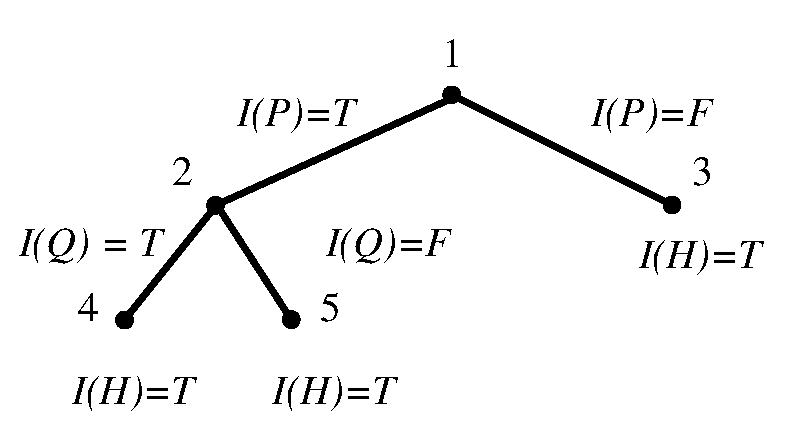
\includegraphics[width=0.7\textwidth]{images/04/tree_01.eps}
    \end{tabular}
  \end{center}
  %\caption{\label{fig:tree:01}}
\end{figure}

\clearpage

\begin{easylist}
  & Exemplo: seja $H = \; (P \OR \NOT Q) \BIC (\NOT P \IMP \NOT Q)$, demonstre que $H$ é uma tautologia usando o método da árvore semântica.
\end{easylist}

\begin{center}
  \begin{tabular}{ c|cccccccccc }
        & $(P$ & $\OR$ & $\NOT$ & $Q)$ & $\BIC$ & $(\NOT$ & $P$ & $\IMP$ & $\NOT$ & $Q)$ \\
    \hline
      2 & $T$  & $T$   &        &      & $T$    & $F$     & $T$ & $T$    &        &      \\
    \hline
      3 & $F$  &       &        &      &        & $T$     & $F$ &        &        &      \\
    \hline
      4 & $F$  & $F$   & $F$    & $T$  & $T$    & $T$     & $F$ & $F$    & $F$    & $T$  \\
    \hline
      5 & $F$  & $T$   & $T$    & $F$  & $T$    & $T$     & $F$ & $T$    & $T$    & $F$  \\
  \end{tabular}
\end{center}

\begin{figure}[!h]
  \begin{center}
    \begin{tabular}{c}
      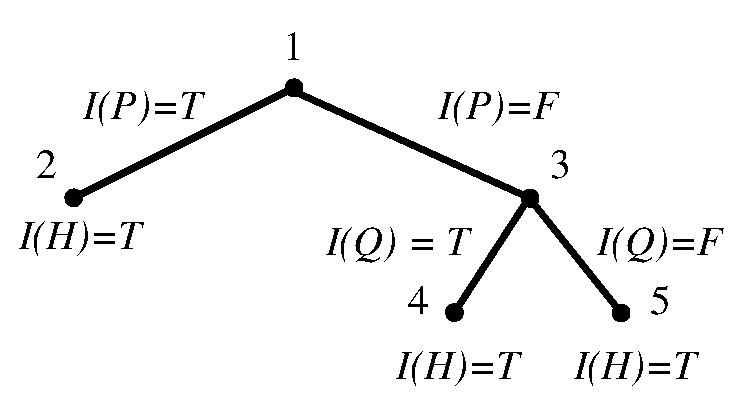
\includegraphics[width=0.7\textwidth]{images/04/tree_02.eps}
    \end{tabular}
  \end{center}
  %\caption{\label{fig:tree:01}}
\end{figure}


